
\chapter{Inferring the connectivity of a mouse's neuronal system}

In chapter 4 a neural network model was simulated to try and mimic the behaviour of the real network described in \ref{sec:mouse_dataset}. A new input stimulus and two cascade generation methods were proposed. In this chapter, the suitability of these new methods will be proved by inferring the connectivity of the new simulation model outlined in section \ref{sec:input_stimulus}. Moreover, the effect of the simulation duration and the network size on the performance of the algorithm will be assessed.\\

Once the suitability has been demonstrated, the same algorithm will be used to infer the connectivity of one of the networks from the CRCNS dataset. Further analysis of this structure will be carried out and its main characteristics will be described.\\

In order to evaluate the performance of the algorithm, the four metrics described in \ref{sec:performance_metrics} will be used. However, as outlined in \cite{pranav_report}, the structure of the network can have a great effect on NetRate's ability to estimate it. For this reason, for validating the suitability of the model, an average of 4 experiments will be used as the results displayed in this chapter.

\section{Proof of the suitability of the algorithm}\label{sec:proof_suitability}


\section{Effect of the size of the network and simulation time on the performance of NetRate}

It is of interest to analyse how the performance of the algorithm varies with different simulation times. Figure \ref{fig:results_10_neurons} shows the results for this analysis. It can be observed that the larger the simulation time, the better NetRate's ability to infer the network. This finding is to be expected due to the fact that the longer the observation length, the more information is captured. However, this behaviour begins to plateau after 1250 seconds of simulation time.\\

\begin{figure}
	\centering
	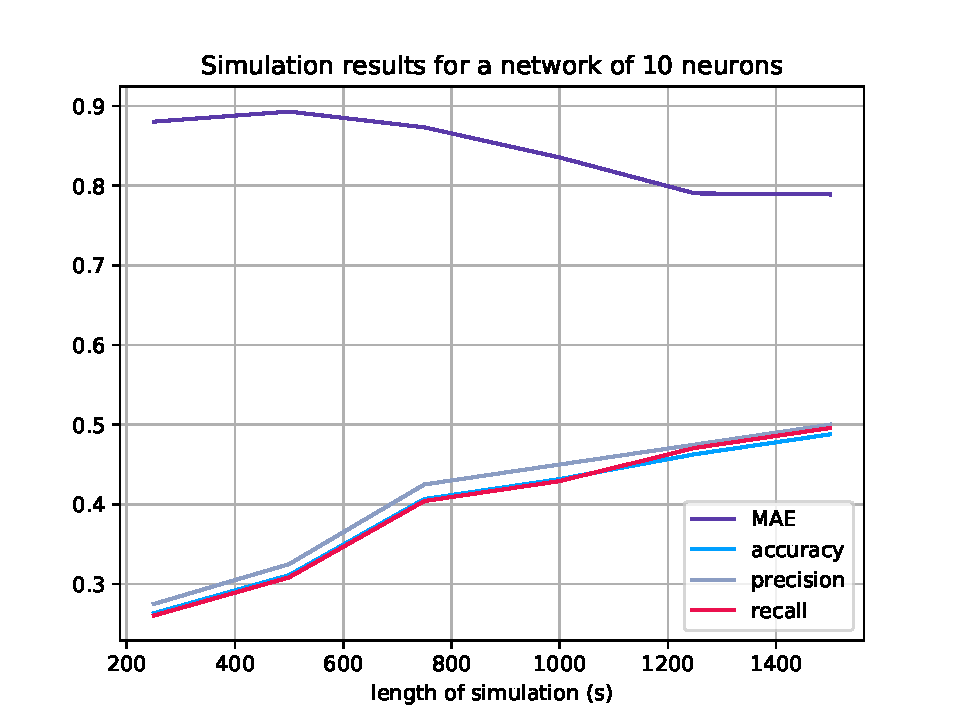
\includegraphics[width=0.8\linewidth]{results_10_neurons.pdf}
	\caption{Network inference performance for a neural network of 10 neurons}
	\label{fig:results_10_neurons}
\end{figure}




\begin{figure}
	\centering
	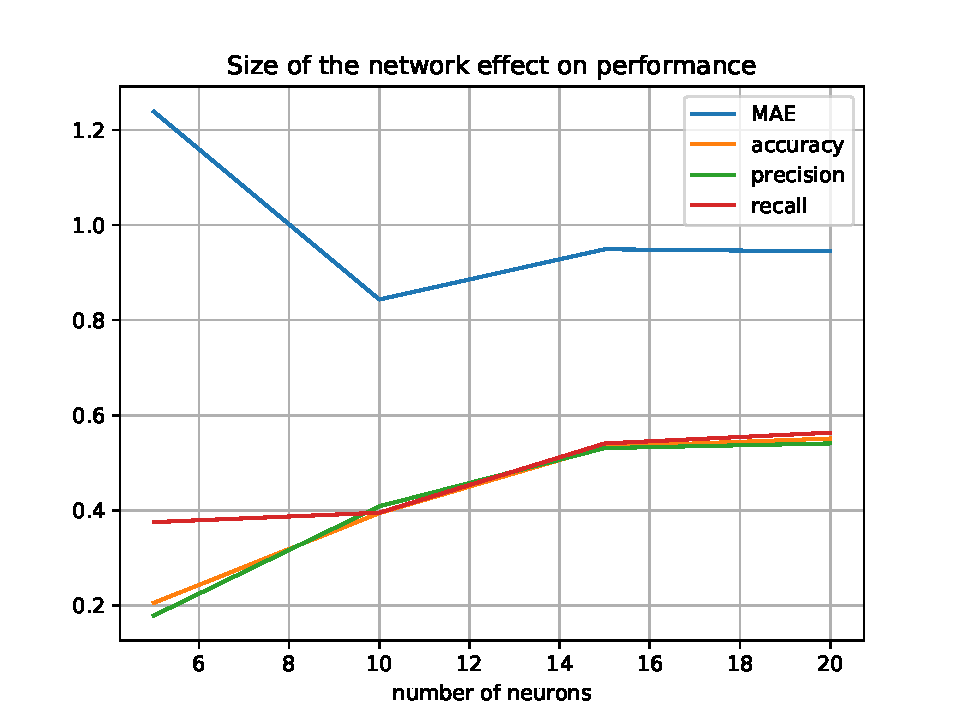
\includegraphics[width=0.8\linewidth]{size_effect_performance.pdf}
	\caption{Average network inference performance for different network sizes}
	\label{fig:results_network_sizes}
\end{figure}

\section{Evaluating the performance without a ground truth}
\section{Inference results}

Once the suitability of the algorithm has been proven, the connectivity of a biological neural network can be inferred. In this section, the 98 neuron network analysed in section \ref{sec:mouse_dataset} and whose evaluation suitability was proven in \ref{sec:proof_suitability} is the one evaluated. Due to the dataset being large enough, the \textit{optimal independence} method of cascade generation is employed. As explained in section \ref{sec:optimal_independence}, this will achieve a higher quality set of cascades.\\

When computing NetRate for a large dataset like the one at hand, the main constraint that the researcher has to deal with is memory. This is directly proportional to the number of cascades computed at any given moment. Therefore, if only one processor is being used, the constraint will be set by the node with the maximum number of cascades. For the current dataset and, using the \textit{optimal independence} method of cascade generation, this corresponds to neuron 12 with 7956 cascades. The computation of this node requires an array of size 18Gb but, with the resources at hand, such an operation is not possible. For this reason, the dataset is partitioned into a smaller set containing the first half of the spike recordings. If the system is assumed to be static\footnote{A network is static if no connections are created or erased during the period of observation.} for the whole length of the recording, then only the performance of NetRate could be affected by this split. The resulting maximum number of cascades is reduced to 5168, with the amount of memory required being lowered to 11Gb.\\

In figure \ref{fig:crcns_4_network}, the resulting inferred network is displayed. Each of the nodes is represented by a circle whose connections are the lines adjacent to them. Since the network is directed, the edges are represented by arrows that indicate the source and target of the connections. Each of the nodes in the figure is coloured according to their degree. Nodes in directed networks can be described by their indegree and outdegree i.e., number of inward and outward connections, respectively. Red nodes have more inward connections and blue nodes more outward connections. If their inward and outward degree is the same, in the figure, these cancel out and their colour becomes purple, just like neurons that have no connections at all. \\

\begin{figure}
	\centering
	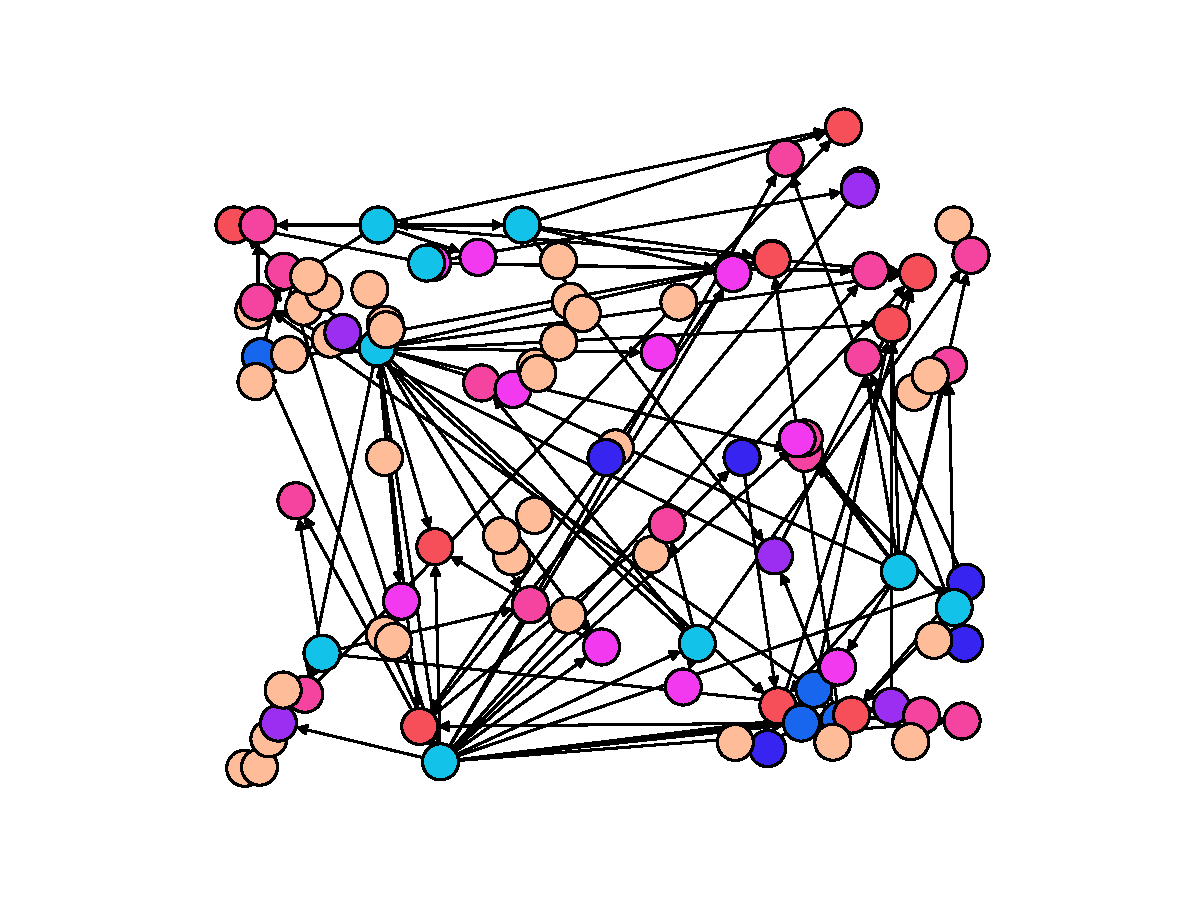
\includegraphics[width=0.8\linewidth]{crcns_4_50_xy.pdf}
	\caption{Inference of a biological neural network of 98 neurons. Red for indegree > outdegree, blue for outdegree > indegree and peach for non connected neurons.}
	\label{fig:crcns_4_network}
\end{figure}

\begin{figure}
	\centering
	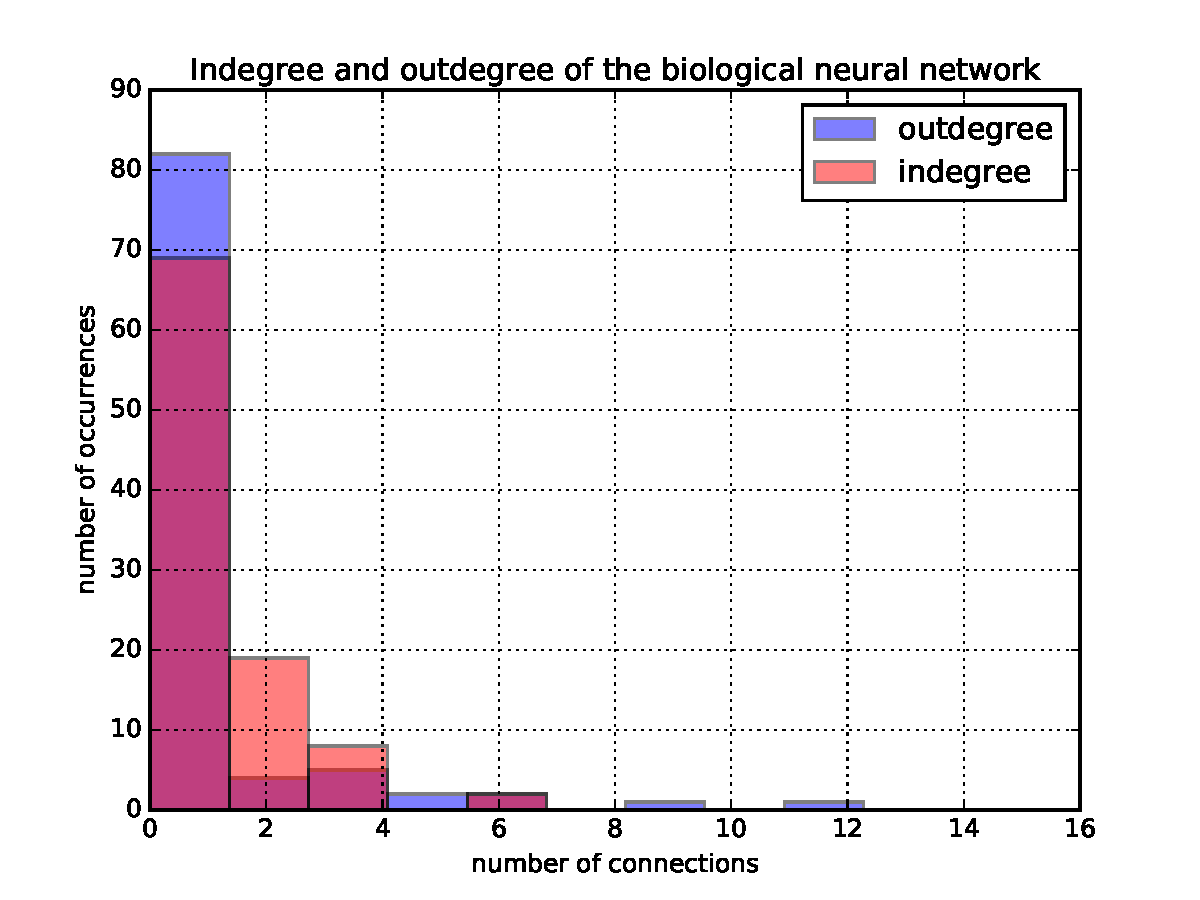
\includegraphics[width=0.8\linewidth]{degree_histogram_real_network.pdf}
	\caption{Indegree and outdegree histogram of a biological neural network}
	\label{fig:degree_histogram}
\end{figure}

An illustration of the degree of nodes in the network is shown in figure \ref{fig:degree_histogram}. As it can be observed, the degree distribution follows an exponential behaviour. Most of the nodes have at least one connection and very few have more. In general, neurons with a greater indegree will spike more often since they are more influenced by their neighbours. This finding agrees with the behaviour of spiking activity shown in figure \ref{fig:histogram_spikes}, where most neurons spike unfrequently and only few have a more intense spiking activity.\\

It is also of interest to analyse whether there exists any dependence between node distance and connectivity. In other words, whether two neurons close to each other have a higher chance of being connected. First, in order to test this hypothesis, the average distance between neurons is calculated. Since the dataset contains the x-y coordinates of all the neurons in the network, it is easy to see that this is equal to 831.57 \(\mu m\). Next, the average edge distance is computed. The value of this calculation is found to be 698.37 \(\mu m\). Although this value is lower than that of the average node distance, the difference is not sufficiently large so as to prove the validity of the hypothesis.








